% -*- mode: fundamental -*-

% ****************************************************************

\chapter{Introduction}

\markboth{Ch \arabic{chapter}: Introduction}{\copyrightnotice}


\setcounter{page}{1}
% \renewcommand{\thepage}{\arabic{page}}
\renewcommand{\thepage}{\arabic{chapter}-\arabic{page}}

\label{ch_intro}

% ****************************************************************

\section{Goals}

\label{Sec_Goals}

This book has two complementary goals, illustrated in Figure~\ref{Fig_Goals}.
\begin{figure}[htbp]
  \centerline{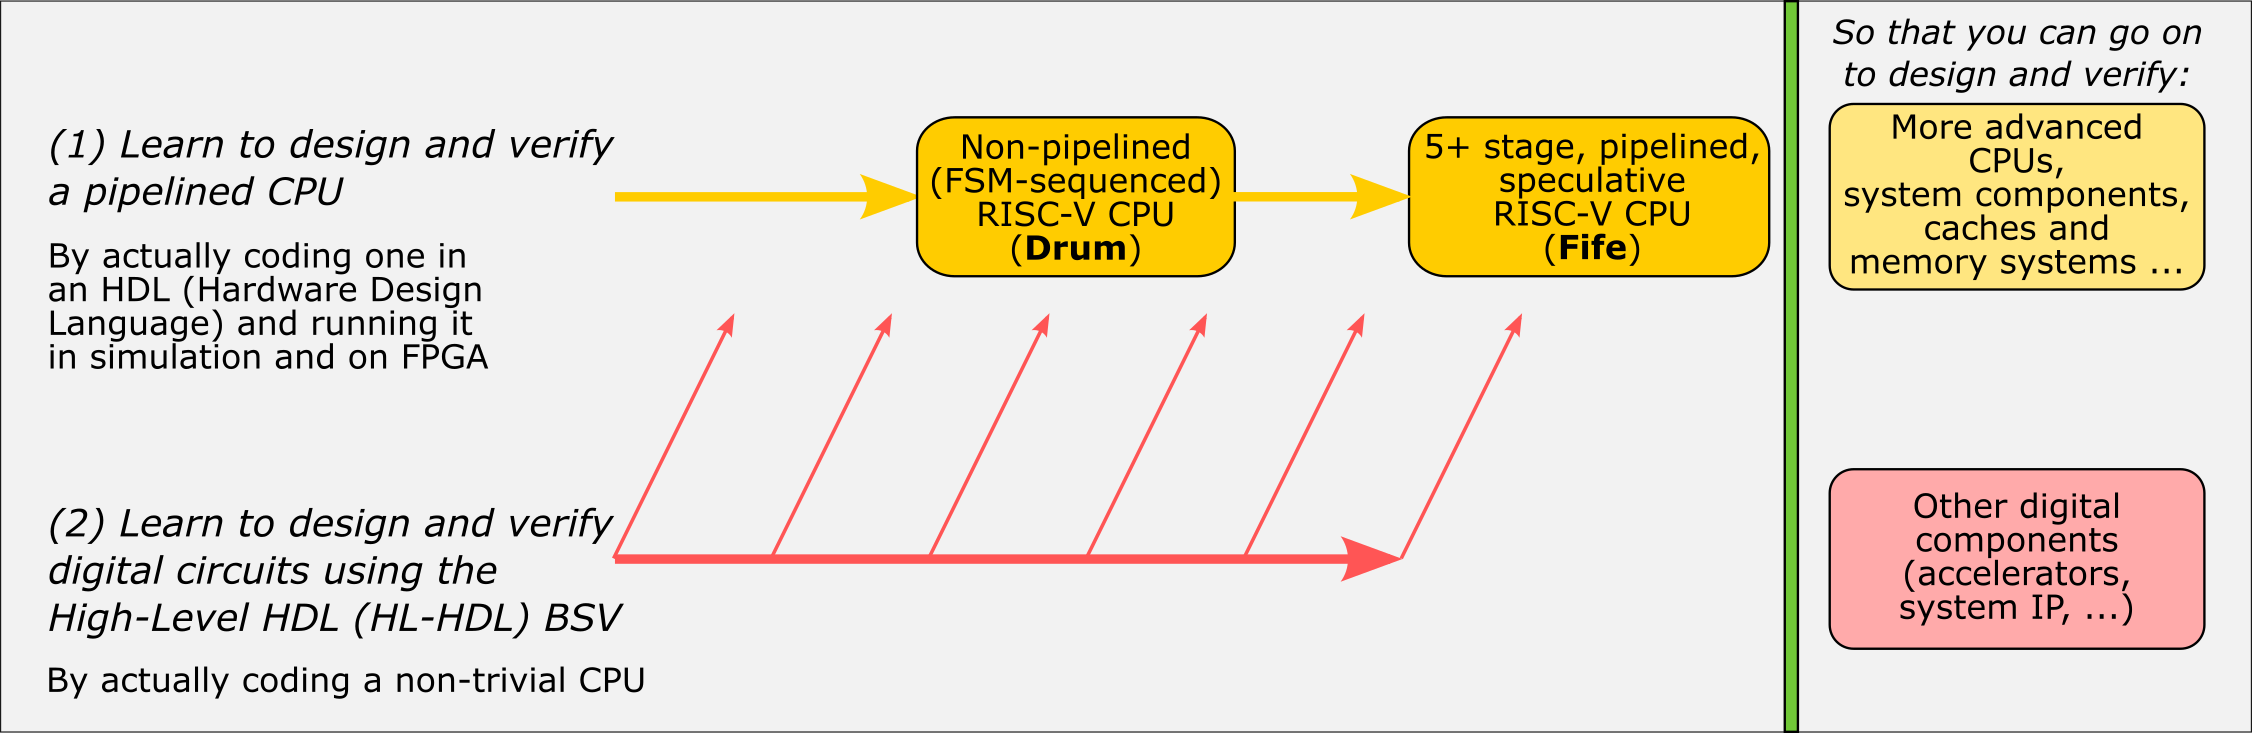
\includegraphics[width=6in,angle=0]{Figures/Fig_Goals}}
  \caption{\label{Fig_Goals}Goals for this book}
\end{figure}

First, the book should help you learn to design a non-trivial computer
processor (CPU).  Second, the book should help you learn modern
digital hardware design, which nowadays is done using a Hardware
Design Language (HDL).

The two goals are nicely complementary.  One cannot really understand
how to design a CPU with just textbook, pencil and paper, and
whiteboard.  For deeper understanding one needs really to \emph{do the
design} and actually run it (in simulation first, on FPGA second, and
possibly finally on ASIC).\footnote{FPGAs and ASICs are certain kinds
of silicon hardware circuit devices.  Appendix~\ref{apx_Glossary} has
a Glossary with more information.}

Similarly, one cannot really learn an HDL (or any progrmming language
for that matter) without actually practising writing, running and
testing programs.  For this, we need interesting examples; what better
example than designing a CPU?

In this book we learn how to design two RISC-V CPUs, \emph{Drum} and
\emph{Fife}, both of which can execute exactly the same RISC-V
binaries ({\ie} RISC-V machine code produced from C programs (for
example) by the \emph{riscv-gcc} compiler (or other RISC-V compilers).

Drum is the simpler CPU. Because it is not pipelined; by designing
this first, we can master all the nuances of RISC-V
\emph{functionality} without being distracted by complexities due to
pipelining.  Then we move on to Fife, where we can focus exclusively
on the complexities due to pipelining.  This is facilitated by the
fact that \emph{Fife reuses most of the RISC-V functional code
developed for Drum}.

Both designs are coded in the BSV High-Level HDL (HL-HDL).  We
interleave topics from BSV and CPU-design so that BSV can be learned
gradually and incrementally.  After each step in learning BSV, we
apply that new knowledge to another actual sub-design of the CPUs.
Each chapter title is prefixed by ``RISC-V'' or ``BSV'' to indicate
whether the chapter is primarily about RISC-V or mostly about BSV.

By the end of this book, we will not only be quite fluent in BSV for
digital design, we will also have two RISC-V CPU designs that we can
run in simulation and on FPGAs, {\ie} which can execute RISC-V
binaries.

Equally important, the student will be ready to move on to more
advanced projects in digital system and subsystem design, including
other CPUs, RISC-V or otherwise, of varying complexity.  Of course,
the topics in this book are just the tip of the iceberg; it takes
years of experience and skill to be able to design a modern, advanced
CPU, but this book should prepare the student well to launch into such
endeavors.  At the end of the book,
Chapters~\ref{ch_BSV_further_study} and \ref{ch_RISCV_further_study}
contain suggestions for further study.

% ****************************************************************

\section{The plan, in more detail}

Figure~\ref{Fig_Topics} shows the broad range of topics that CPU
designer needs to know.  In this book we will touch on all the red
topics.
\begin{figure}[htbp]
  \centerline{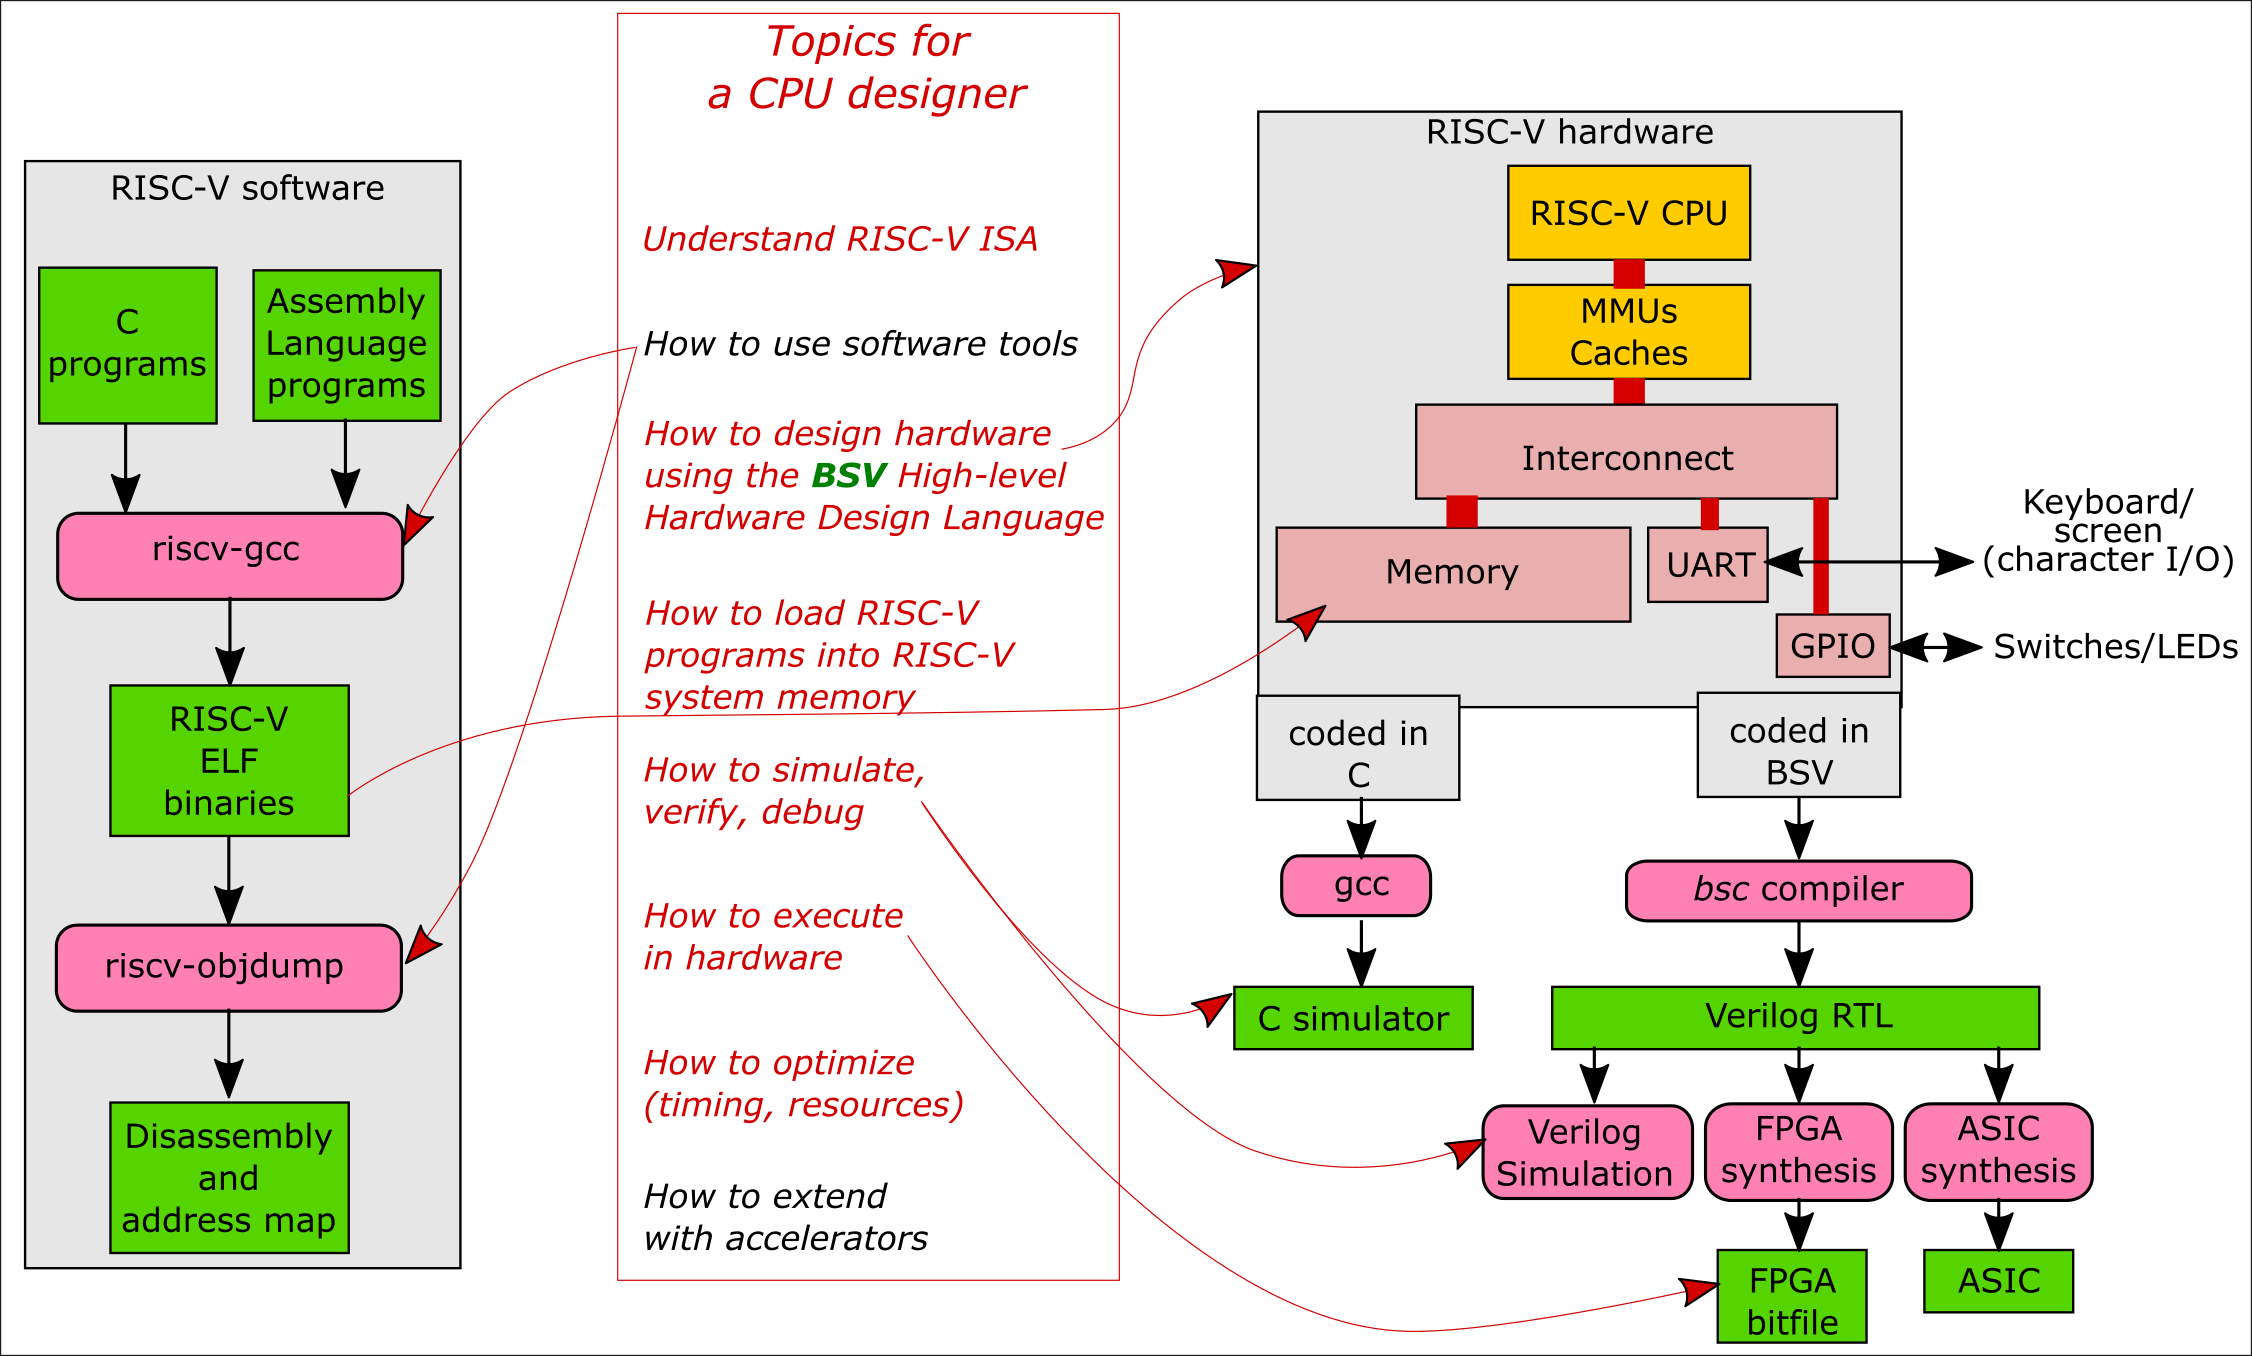
\includegraphics[width=6in,angle=0]{Figures/Fig_Topics}}
  \caption{\label{Fig_Topics}Topics covered in this book (in red text in red box)}
\end{figure}

We start by reviewing the RISC-V ISA itself in Chapter~\ref{ch_ISA}.
What are RISC-V instructions? How are they coded in bits? What does
executing an instruction mean?  The ISA \emph{per se} is not a focus
of this book (for which many textbooks and educational materials are
available), but understanding the ISA is of course a prerequisite to
designing a CPU.

The RISC-V ISA has many options, discussed in Chapter~\ref{ch_ISA};
our focus in this book will be on a small standard subset called
``RV32I'' which is adequate for small embedded systems.

% ----------------

\vspace{1ex}

NOTE: \fbox{\small
\begin{minipage}{5in}

In order to run actual RISC-V programs on our implementations, we need
to undertand how to use the \emph{riscv-gcc} compiler to compile C and
RISC-V Assembly Language programs into RISC-V binaries (so-called
``ELF'' files).  Another useful tool is \emph{riscv-objdump}, which
can disassemble the binary back into assembly-language text. This is
useful for debugging our implementation, so that we can understand
execution instruction-by-instruction, and diagnose anything that goes
wrong.

\vspace{1ex}

\emph{In this book we do not discuss how to install and use these
tools}.

\end{minipage}}

\vspace{1ex}

% ----------------

Most of the book is focused on designing and verifying Drum and Fife.

We code our designs in BSV.  We use BSV for CPU itself, and for the
top-level testbench.  For simulation, the supporting ``system''
components---a Memory, UART and GPIO---are written in C and linked
into the simulation executable.  For running on FPGA the supporting
system components use some existing hardware infrastructure.

We use the \emph{bsc} compiler to translate BSV code into Verilog RTL.
We simulate the generated Verilog in Verilator, a free and open-source
Verilog simulation system (the generated Verilog can also run on any
other Verilog simulator).

Verilog simulation provides an exact, cycle-by-cycle accurate
simulation of the very same design that we run later on an FPGA.
Simulation is invaluable for debugging the hardware design because the
turnaround time to fix a problem and run a new simulation is very
short (minutes) compared to creating a new version for an FPGA
(several hours).

Of course, Verilog simulation runs much more slowly (10,000x or
slower) compared to an FPGA, and so simulation is useful primarily for
early debugging and analysis of the design, running small RISC-V
programs.

In Chapters~\ref{ch_BSV_verification}, \ref{ch_RISCV_verification},
and \ref{ch_Optimization} we discuss debugging and optimization of our
RISC-V designs, in particular using \emph{traces} that are generated
during simulation.

We will discuss how to process our Verilog RTL through an FPGA
synthesis tool to create an FPGA bitfile which can then be loaded into
an FPGA and executed in hardware.  We will use FPGAs in the Amazon AWS
cloud, but it can be synthesized and run on any other FPGA platform as
well.

% ----------------

\vspace{1ex}

NOTE: \fbox{\small
\begin{minipage}{5in}

Our Verilog RTL can also be processed through ASIC synthesis tools
targeting ASIC fabrication.  We will not be discussing ASIC flows in
this book.

\end{minipage}}

\vspace{1ex}

% ----------------

% ****************************************************************

\section{Drum and Fife, our two implementations}

\label{Sec_Drum_and_Fife}

% ================================================================

\subsection{The Design Space for CPU implementations}

\label{Sec_Interpreters}

Any artefact/engine that executes the instructions of any ISA is an
\emph{interpreter} for that ISA.  Interpreters can be implemented in
software or in hardware.

ISA interpreters written in software, and running like any other
program on workstations, are called ``simulators''.  We do not discuss
them in this book, although we may use them during verification of our
hardware designs.  Appendix~\ref{apx_resources_trusted_simulators} has
more information on, and references to open-source RISC-V simulators.

Hardware implementations (and even software simulators) can vary
widely in microarchitecture.  Some design options are:

\begin{itemize}

  \item Sequential or pipelined?  One full instruction at-a-time, or
    multiple instructions flowing through a pipe, each at a more
    advanced stage in its execution than the one behind it?

  \item Predictive? In pipelined implementations, can we predict what
    instructions to fetch while a BRANCH/JUMP flows through the pipe,
    before we know the actual next-instruction determined by the
    BRANCH/JUMP?

  \item Superscalar/VLIW? Fetch and execute more than one instruction
    in parallel, taking care to preserve sequential ISA semantics?

  \item Out-of-order? Execute each instruction as soon as its input
    data is available, without waiting for prior instructions which
    may still be waiting for their inputs?

\end{itemize}

For the same microarchitecture, a software simulator is typically
\emph{much slower} than a hardware implementation (often by factors of
tens of thousands).  This is because it involves (at least) two layers
of simulation. The software simulator is itself a program that is
being interpreted by the underlying workstation hardware.  That
program (the simulator), in turn, is interpreting the target ISA.
Every layer of interpretation can slow down overall performance by
an order of magnitude or more.

Paradoxically, adding microarchitectural detail will normally slow
down a software simulator but speed up a hardware implementation.
This is because more microarchitetural detail usually exploits more
\emph{parallelism} and \emph{concurrency} in RISC-V interpretation,
which can be fully exploited by hardware, but requires more sequential
work in a software simulator.

% ================================================================

\subsection{ISA executed by Drum and Fife}

Drum and Fife execute exactly the same binaries; the only difference
will be in Fife's superior performance (speed).

As described in more detail in Chapter~\ref{ch_ISA}, the RISC-V ISA
has many modular options.  For Drum and Fife, we limit our attention
to a small subset:

\begin{itemize}
		  
 \item The so-called ``RV32I'' ISA from the RISC-V Unprivileged ISA
       spec: basic integer arithmetic and logic operations; branch and
       jump; load and store.

 \item Plus: a few elements from the RISC-V Privileged ISA spec for
       handling exceptions: Control and Status Registers (CSRs), traps
       and trap-handling, and CSRRxx instructions.  This allows
       software to recover from illegal instructions, memory access
       errors, and so on.

\end{itemize}

For detailed information on RV32I, please see the specification
document ``The RISC-V Instruction Set Manual Volume I: Unprivileged
ISA''~\cite{RISCV_Unpriv_2019_12_13}.  In particular, look at:

\begin{itemize}

 \item The first table in Chapter 24 ``RV32/64G Instruction Set
       Listings'' entitled ``RV32I Base Instruction Set'', showing the
       forty RV32I instructions (and reproduced in
       Figure~\ref{Fig_RV32I_labeled}).

 \item These instructions are described in more detail in that
       document in Chapter 2 ``RV32I Base Integer Instruction Set,
       Version 2.1''.

\end{itemize}

For detailed information on traps and trap-handling, please see the
specification document ``The RISC-V Instruction Set Manual Volume II:
Privileged Architecture''~\cite{RISCV_Priv_2021_12_03}.

% ================================================================

\subsection{Drum and Fife}

Drum and Fife are illustrated in
Figure~\ref{Fig_Two_Microarchitectures}.  Each instruction is taken it
through the stages shown.
\begin{figure}[htbp]
  \centerline{\includegraphics[width=6in,angle=0]{Figures/Fig_Two_Microarchitectures}}
  \caption{\label{Fig_Two_Microarchitectures}Two CPU implementations (microarchitectures)}
\end{figure}

Drum is a \emph{non-pipelined} implementation.  For each instruction,
the design is FSM-sequenced through the stages shown in the diagram,
completing all stages sequentially before starting on the next
instruction.

Drum is almost a direct transliteration into BSV code of the generic
ISA execution algorithm described in
Section~\ref{Sec_ISA_Exec_Algorithm}.  In fact the BSV code will look
very similar C/C++ code for a purely functional RISC-V simulator.
Being written in BSV, however, we can compile and run it on actual
hardware (FPGAs, ASICs).
       
The design of Drum will familiarize us with all the basic RISC-V
concepts and execution flows (the RISC-V ISA, preparing and running a
RISC-V binary to run on the design, analysing traces), without being
distracted by the complexities of pipelining.

Drum is not fast compared to Fife or other hardware CPUs, because of
its lack of microarchitectural features, but we can still synthesize
it to run at several 100 MHz on an FPGA, which makes it faster than
most software functional simulators.  It will be small (silicon area,
and therefore low power as well).

Drum is covered in Chapter~\ref{ch_core_functions} through
Chapter~\ref{ch_Drum_code}.

Fife is a 5+ stage pipelined design, which is a microarchitectural
change focused on higher performance (speed) than Drum.  All the
stages in the diagram run \emph{concurrently}, with each stage
receiving input from the previous stage to its left (``upstream'') and
producing output for the next stage to its right (``downstream'').
The design includes simple branch-prediction, register read/write
hazard management, concurrent execution pipelines, in-order retirement
of instructions, and speculative stores to memory using a
store-buffer.

Fife is covered in Chapter~\ref{ch_Fife_Principles} through
Chapter~\ref{ch_Fife_code}.

Fife \emph{reuses} most of the RISC-V functional code from Drum
without change.  Thus, Fife chapters can focus purely on the new
issues raised by pipelining (and which are in fact applicable to any
pipelined CPU design, not just RISC-V).

At the end of the book, Chapter~\ref{ch_RISCV_further_study} discusses
how to extend Drum and Fife to handle RV64I and more Unprivileged ISA
options---M: integer multiply/divide, A: atomics, FD: single-and
double-precision floating point, and C: compressed--- and more
privileged ISA options---Privilege levels (M: Machine, S: Supervisor
and U:User; full complement of Control and Status Registers (CSRs);
Virtual Memory).  With these extensions, Drum and Fife will be able to
run a full-feature Operating System (OS), such as Linux.

% ================================================================

\subsection{Drum and Fife source codes}

The full source codes (BSV) for Drum and Fife are included with this
book.  Excerpts of the actual code are taken, as-is, for inclusion in
this book.  Excerpts look like this:

\SHOWCODE{Code_Extracts/CPU_IFC.tex}

The label on the top border of the box indicates file
(\verb|src_Common/CPU_IFC.bsv|) from which this has been excerpted,
and the starting line number (27) in the file.  The ``\verb|...|''
indicates we have \emph{elided} some lines from the source file which
are not directly relevant to the current discussion.

We recommend, as you read the book, that you also keep open a text
editor in which you can simultaneously view the actual sources.

% ****************************************************************

\section{About BSV, the HL-HDL we use for our designs}

Both designs are coded in BSV, a free, open-source, modern, High-Level
Hardware Design Language (HL-HDL).  BSV code can be compiled into
Verilog, which can then be run on any Verilog simulator, or can be
further processed by FPGA tools to run on FPGAs, or by ASIC tools for
ASIC implemenetations.

\index[BSV]{BH (alternate Haskell-like syntax)}
\index[BSV]{Haskell!Influence on BSV}
\index[BSV]{Haskell!BH alternate Haskell-like syntax for BSV}

BSV is a modern, high-level HDL taking inspiration from two sources in
modern software programming languages.  First, for data types, program
structure, and static elaboration, BSV directly emulates the Haskell
functional programming language.  In fact, BSV is actually Haskell,
with a syntax closer to SystemVerilog.  For Haskell enthusiasts, there
is an alternate syntax called ``BH'' which directly uses Haskell
syntax; please see \emph{bsc} documentation for details.

For specifying dynamic behavior, BSV emulates a class of formal
specification languages for concurrent programming based on rules
(including Term Rewriting Systems, Unity, TLA+, and Event-B).

BSV is a ``universal'' digital hardware design language, like Verilog
and SystemVerilog.  Although here we focus on CPU design, it is
suitable for any digital hardware design whatsoever.

Appendix~\ref{apx_Why_BSV} has a more detailed justification of why we
choose BSV over other hardware design languages like Verilog,
SystemVerilog and VHDL.

% ****************************************************************

\section{Basic model of digital hardware needed for this book}

``Digital Design'' is traditionally taught as a separate course
preceding any course on CPU design.  Much time is spent on circuit
diagrams and schematics, then transitioning to hardware design
languages (HDLs) like Verilog, SystemVerilog or VHDL.  Topics include
boolean logic gates (AND, OR, NOT, XOR, ...), combinational circuits
(half-adders, adders, multiplexers, ...), logic minimization, flip
flops, registers, binary number representations (twos complement),
FSMs (Finite State Machines), and so on.  Supporting examples are
often quite artificial and simplistic.

However, just like the transition in software programming languages
from machine code and assembly language to high-level languages (which
began in the 1960s and 1970s), most modern digital hardware design is
done at a higher level of abstraction.  Designs are described using
HDLs like Verilog, SystemVerilog and VHDL.  We express logic using
traditional arithmetic and logic operators on bit-vectors; we express
multiplexes using if-then-else and case statements; we use library
elements for $n$-bit registers, FIFOs, memories, and so on.  We rely
on \emph{compilers} (synthesis tools) to transform such descriptions
into low-level gates, wires, flip-flops, {\etc}.

Accordingly, we will focus here on BSV language-based hardware design,
and skip the study of detailed low-level underlying circuits.  All our
examples will be taken from Drum and Fife so that the motivation is
clear.

In the next few sections, we cover the basic digital hardware concepts
that are adequate to launch us into designing Drum and Fife with BSV.

% ================================================================

\subsection{Clocks and State Elements}

Digital hardware is driven by a clock, an electrical signal that
oscillates between a low voltage and a high voltage, with sharp
transitions between the two, at regular intervals (it is therefore
sometimes called a ``square'' wave).  This is illustrated in
Figure~\ref{Fig_Clock_1}.

\begin{figure}[htbp]
  \centerline{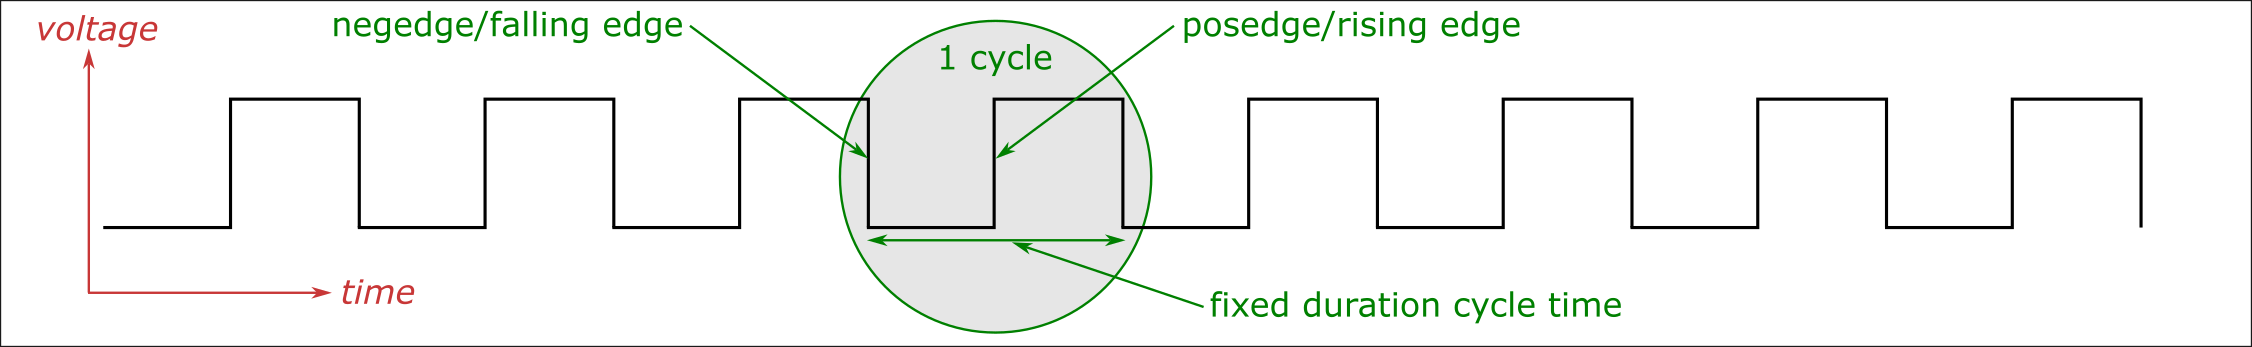
\includegraphics[width=6in,angle=0]{Figures/Fig_Clock}}
  \caption{\label{Fig_Clock_1}A clock signal}
\end{figure}

Nowadays, clock cycle times/periods are typically measured in
nanoseconds. For example, a 100 MHz clock has a 10ns cycle time.

\index[BSV]{State elements}

Any value that must be visible from one clock to the next must be
\emph{stored} in a \emph{state element}---a component that can
``remember'' values, {\ie} has \emph{state}, like a register, FIFOF,
buffer, memory, ....

% ================================================================

\subsection{Bit-vectors, values and buses}

\index[BSV]{Bit-vector}
\index[BSV]{bus}
\index[BSV]{values!abstract entity coded in bits}

All data in digital circuits are represented in binary form, as
vectors of bits.  In BSV notation, the \emph{type} (data type) of a
bit-vector is written like this: ``{\tt Bit\#($n$)}'', where $n$ is
the number of bits (width of the bit-vector).  A bit-vector may
directly represent bits, or it may be an encoding of some higher-level
construct such as an instruction, a register name, a character string,
a memory request or response, and so on.  Collectively we call all
such constructs \emph{values}.

In hardware, values are carried on bundles of wires called
\emph{buses}.  In circuit diagrams, an $n$-bit-wide bus is usually
drawn as a line with a small diagonal hash mark labeled with $n$.
Values are also stored in state elements.

% ================================================================

\subsection{Digital circuits}

\index[BSV]{Combinational circuits}

Digital circuits are composed of state elements and
\emph{combinational circuits} connecting outputs of state elements to
inputs of state elements, as illustrated in
Figure~\ref{Fig_BSV_Digital_Circuits}.
\begin{figure}[htbp]
  \centerline{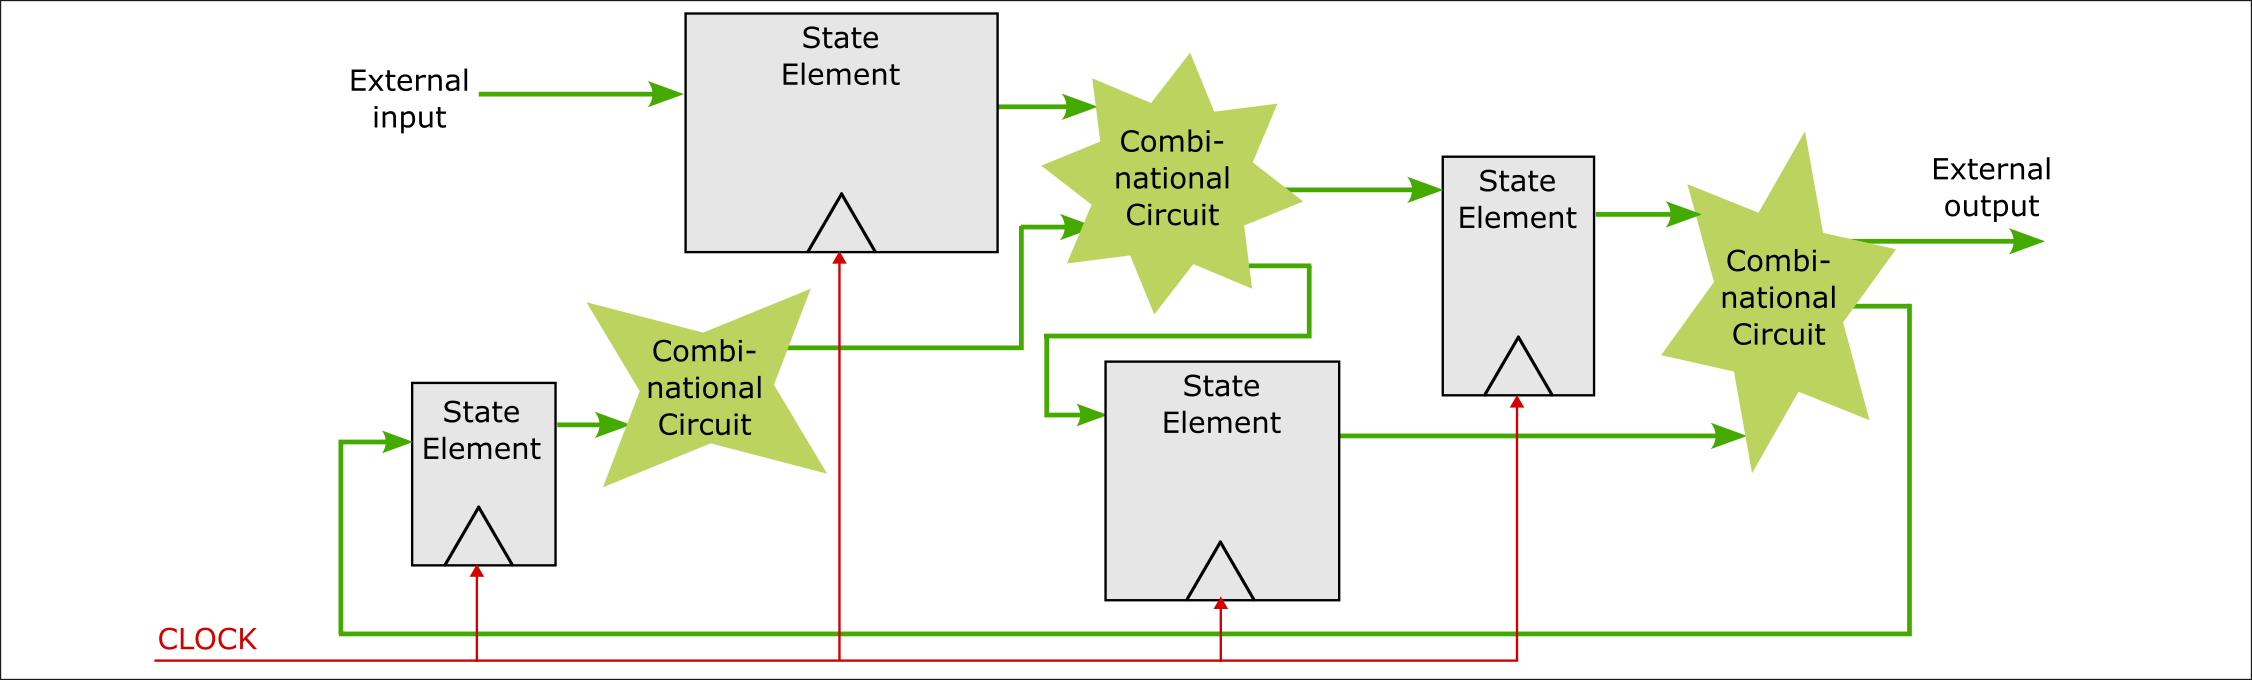
\includegraphics[width=6in,angle=0]{Figures/Fig_BSV_Digital_Circuits}}
  \caption{\label{Fig_BSV_Digital_Circuits}
           Digital circuits consist of state elements interconnected
	   with acyclic combinational circuits}
\end{figure}

State elements are \emph{storage} elements.  Combinational circuits
are \emph{acyclic} networks of \emph{logic gates}.  A logic gate is a
circuit that ``instantaneously'' computes an output boolean value that
is a function of its boolean inputs (such as AND, OR, NOT, XOR, ...).

Any digital circuit repeatedly performs the following:

\begin{itemize}

\item After each ``posedge'' (positive edge of a clock), the
      combinational circuits compute new input values for all state
      elements, based on the current output values from state elements.

\item At the next posedge, these new input values are stored into
      (``clocked into'') the state elements.

\end{itemize}

The above description is a simplification, or an idealization.
Physics and circuit silicon technology dictates how long an electrical
signal takes to propagate from the output of a state element and
through a combinational circuit before it arrives at the input of a
state element.  For correct operation, the clock period needs to be
greater than this, to allow signals that are inputs to state elements
to ``settle down'' and be steady when they are captured on the next
clock edge.

\index[BSV]{Digital Abstraction, The}

In the \emph{Digital Abstraction} we assume this condition is met, and
we idealize wire and combinational circuit delays as taking zero time.

% ----------------

\vspace{1ex}

NOTE: \fbox{\small
\begin{minipage}{5in}

\begin{itemize}

 \item Advanced digital ciruits may have multiple clocks driving
       different parts of the circuit.

 \item Advanced digital ciruits may vary the clock speed dynamically,
       to match power consumption to current performance demands
       (higher speeds $\Rightarrow$ more power consumption).

 \item Some digital ciruits use the negative edge (``negedge'') of the
       clock insted of the posedge.

 \item Advanced digital ciruits may use both the posedge and the
       negedge of the clock.

\end{itemize}

\end{minipage}}

\vspace{1ex}

% ----------------

% ================================================================

\subsection{Computer memories}

\label{Sec_mem_split_phase}

\index[BSV]{Memory}

A computer memory is a packaged sub-system:
\begin{itemize}

 \item To read memory, we present a \emph{read request} at its inputs,
       with an \emph{address}; \\
       the memory provides a \emph{read response} at its outputs,
       containing the addressed data.

 \item To write memory, we present a \emph{write request} at its
       inputs, with an address and data; \\
       the memory provides a \emph{write response} at its outputs,
       containing an ``ok'' status.

\end{itemize}

\index[BSV]{RAM (Random Access Memory)}
\index[BSV]{Memory!RAM (Random Access Memory)}

Because we access memory by presenting an address identifying a
location in memory, they are called RAMs (Random Access Memories).
Nowadays memories are typically byte-addressed, {\ie} each address
identifies a distinct byte in memory.  Memory access instructions in
the CPU (LOAD, STORE) typically specify a \emph{size}, such as 1, 2, 4
or 8 bytes, indicating the number of bytes to transfer between the CPU
and memory.

% ----------------------------------------------------------------

\subsubsection{Memory hierarchies}

\index[BSV]{Memory!Hierarchy}
\index[BSV]{Memory!L1 cache, level 1 cache}
\index[BSV]{Memory!L2 cache, level 2 cache}

Figure~\ref{Fig_Mem_Hierarchy} illustrates a typical memory hierarchy
in a modern computer system.
\begin{figure}[htbp]
  \centerline{\includegraphics[width=6in,angle=0]{Figures/Fig_Mem_Hierarchy}}
  \caption{\label{Fig_Mem_Hierarchy}
           A typical memory hierarchy in a computer system}
\end{figure}
The L1 cache (``Level 1 cache''), L2 cache and Main Memory are all
memory subsystems.  The memory closest to the CPU (L1 cache) is the
smallest, fastest (see Section~\ref{Sec_mem_latency}) consumes most
power and is the most expensive.  The memory furthest from the CPU
(Main Memory) is largest, slowest, consumes least power, and is the
cheapest.

Main Memory contains ``all the real contents'' of memory.  The caches
contain temporary copies of a subset of locations of Main Memory.

\index[RV]{Cache!hit/miss}

The CPU sends its memory request to the L1 cache; if it contains a
copy of the requested address, this is called a ``cache hit'', and the
L1 cache returns the response to the CPU.  If it does not contain a
copy of the requested address (a ``cache miss''), the L1 cache, in
turn, requests it from the L2 cache which, again, may hit or miss.  In
the worst case, a request has to be serviced from Main Memory.  When a
cache retrieves a datum from a lower-level element, it retains it, so
that a future access to the same address will hit.

\label{Sec_mem_latency}

\index[BSV]{Memory!latency (cycles/ticks)}
\index[BSV]{Memory!access latency (cycles/ticks)}
\index[RV]{Cache!Miss penalty}

The delay from when the CPU issues a request until it receives the
corresponding response is called \emph{memory latency}.  This is
typically measured in clock cycles (ticks) or in real-time units
(nanoseconds, microseconds).  L1 caches can typically be accessed in 1
tick if there is a hit.  A cache miss can take up to several tens of
ticks (the so-called ``miss penalty'')..

Memory latency is generally not predictable---it can depend on the
address of the request, and on past history of accesses which affects
what is currently available in the caches.  It can also depend on
technology replacement: next year's memory system may be slower/faster
than today's.

Fortunately, many (if not most) programs exhibit reuse, temporal and
spatial \emph{locality}. Reuse and temporal locality means that an
instruction or datum read from memory is likely to be accessed again
soon.  Spatial locality means that after an instruction or datum is
accessed from an address in memory, the CPU's next accesses are likely
to be from nearby addresses.  These properties increase the likelihood
that a near-future access will hit in the cache and be serviced
quickly.  Modern caches can achieve hit rates (the ratio of hits to
hits+misses) that can approach 90\% or more.

A CPU design should generally not depend on any specific memory
latency, {\ie} it should be robust to changes and variations.

\index[BSV]{Memory!bandwidth}

The rate at which requests and responses can be pumped through the
memory system by the CPU is called \emph{memory bandwidth}.  This is
usually measured in transactions-per-second, or requests-per-second,
or in bytes-per-second where the bytes usually refer to data bytes
transferred, excluding address bytes and other overhead bytes.

% ----------------------------------------------------------------

\subsubsection{Memory technologies for the memory hierarchy}

\index[RV]{SRAM (Static RAM)}
\index[RV]{DRAM (Dynamic RAM)}

\index[RV]{Memory!SRAM (Static RAM)}
\index[RV]{Memory!DRAM (Dynamic RAM)}

Two major categories of memory technologies are SRAMs (Static Random
Access Memories) and DRAMs (Dynamic Random Access Memories).  For the
same size, SRAMs are more expensive (more silicon area, more power
consumption) and faster (less time to access a location) compared to
DRAMs.  Thus, computers typically use SRAMs for L1 caches and DRAMs
for main memory. L2 and other intermediate caches may use SRAM or
DRAM.  Cache sizes typically range from the 10s of kilobytes to 100
megabytes, whereas main memories can range into several gigabytes.

% ----------------------------------------------------------------

\subsubsection{Split-phase memory access}

\index[RV]{Split-phase memory access}
\index[RV]{Split-phase memory transaction}

\index[RV]{Memory!split-phase access}
\index[RV]{Memory!path viewed as a pipeline/queue}

Because memory latency is unpredictable by the CPU, we always assume
memory accesses are \emph{split-phase} transactions---a request action
followed an unpredictable number of ticks later by a response action.
This is illustrated in Figure~\ref{Fig_BSV_Split_Phase_Mem}.
\begin{figure}[htbp]
\centerline{\includegraphics[width=6in,angle=0]{Figures/Fig_BSV_Split_Phase_Mem}}
\caption{\label{Fig_BSV_Split_Phase_Mem} Split-phase memory access}
\end{figure}
During the interval between request and response, the CPU need not be
idle; it can execute other instructions, prepare the next memory
access, {\etc}.

% ----------------------------------------------------------------

\subsubsection{Memory pipelining and memory ordering}

Memory systems are also often pipelined: the CPU can issue a
continuous stream of requests, and the the memory sends back a
continuous stream of responses.  The CPU does not have to wait for a
memory response before issuing the next request.  Thus, in
Figure~\ref{Fig_BSV_Split_Phase_Mem}, we have labeled the arrows to
and from memory with little red symbols representing \emph{queues} or
FIFOs (First-In-First-Out).  The whole path from the CPU to memory and
back can be regarded as a queue, with requests entering and responses
exiting the queue.

% ----------------

\vspace{1ex}

NOTE: \fbox{\small
\begin{minipage}{5in}

Advanced memory systems may not be FIFO-like; the CPU may receive
responses in a different order from the original requests, in the
interests of returning a response as soon the data is available,
rather than waiting idly for its turn.

\vspace{1ex}

\emph{In this book we will assume FIFO-like, in-order memory accesses.}

\end{minipage}}

\vspace{1ex}

% ----------------

% ****************************************************************

\section{Additional Resources for this Textbook/Course}

Appendix~\ref{apx_resources} has a detailed listing of resources
(documents and software tools) needed for this book, and for further
reading.

Appendix~\ref{apx_Glossary} contains a Glossary of terms and
abbreviations.

This book also contains:

\begin{itemize}

 \item a detailed index of BSV topics, and
       Chapter~\ref{ch_BSV_further_study} has suggestions for further
       study of BSV;

 \item a detailed index of RISC-V topics, and
       Chapter~\ref{ch_RISCV_further_study} has suggestions for
       further study of RISC-V and CPU design.

 \end{itemize}

% ****************************************************************
